\part{几何}
\chapter{几何的描述}

几何主要可以分为两类, 一种是\textbf{隐式几何 (Implicit Geometry) }, 一种是\textbf{显式几何 (Explicit Geometry) }. 

\section{隐式几何}
隐式几何是对点几何进行的描述, 并不直接给出点的位置. 例如, 对于一个单位球面, 我们可以使用公式$x^2+y^2+z^2=1$进行表示. 我们可以通过函数$f(x,y,z)=0$隐式地定义一个集合. 
几何的隐式表示很难看出来所对应的图形, 但是可以非常轻松的判断一个点是不是在这个图形面上. 隐式几何有以下几种表示方式: 
\begin{enumerate}
	\item 使用数学函数表示, 是一种不直观的表示方法; 
	\item CSG (Constructive Solid Geometry) 表示, 使用一系列基本几何体通过交、并、差等布尔运算得到最终的结果; 
	\item 距离函数 (Distance Function) 表示, 距离函数表现了空间内任意一点到物体的最短距离. 两个距离函数的加和可以得到两个物体融合的中间态. 非常适合在模拟水滴融合中使用. 距离函数中距离为0的平面就是物体平面. 距离函数还可以使用水平集 (Level Set Method) 来离散的表示; 
	\item 分型 (Fractals) 表示, 指的是一个图形的一部分和自己整体相比高度相似, 可以理解为一种递归的形式. 
\end{enumerate}

\section{显式几何}
显式几何通过直接定义几何上的点或者通过把点进行参数映射的方式定义到新的空间 (例如我们可以把$u-v$平面上的点映射到三维空间中) . 显式几何可以轻松的找到所有的点, 但是不好判断空间中任何一个点是否在图形面上. 显式几何常见的表示方式有以下几种: 
\begin{enumerate}
	\item 点云 (Point Cloud) 表示, 使用一系列空间中三维的坐标来表示物体. 点越密集, 所形成的模型效果越好. 一般会使用点云生成三角形面. 
	\item 多面形面 (Polygon Mesh) 表示, 一般使用三角形或者四边形来表示. 描述更加复杂但也是最为常用的方式. 使用Wavefront Object File (.obj) 格式的文件来存储. 在obj文件中定义了顶点坐标, 法线方向以及纹理坐标还有它们之间的关系. 
\end{enumerate}

\chapter{曲线和曲面}
曲线和曲面是常见的几何. 在本章将会着重讲解曲线和曲面的表示以及有关的性质. 

\section{曲线}
我们使用一系列的点去定义一条曲线. 这些控制点描述了曲线的一些性质. 最常见的曲线叫做\textbf{贝塞尔曲线 (B\'ezier Curve) }. 
\subsection{贝塞尔曲线的画法}
\textbf{在三个点的情况下}

在二维情况下, 使用三个控制点画出的贝塞尔曲线称为二次贝塞尔曲线 (quadratic B\'ezier) . 这是由Pierre B\'ezier和Paul de Casteljau提出的算法, 称为de Casteljau算法. 

\begin{figure}[H]
	\centering
	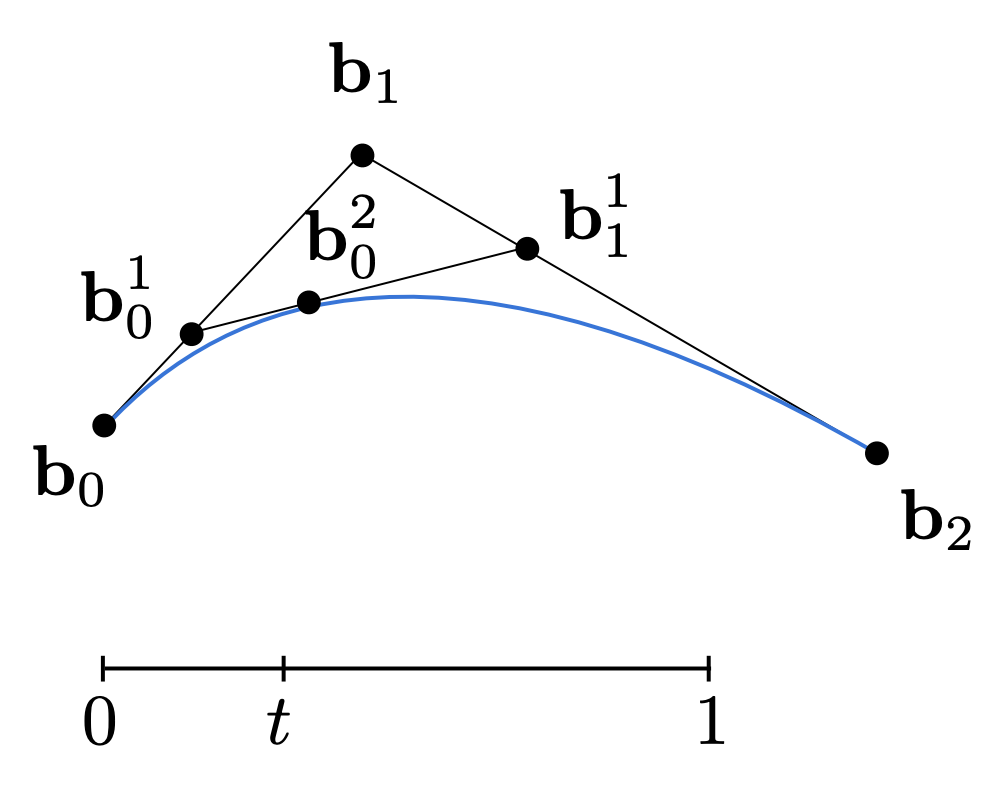
\includegraphics[scale=.3]{beisaier.png}
	\caption{二次贝塞尔曲线的画法}
	\label{fig:beisaier}
\end{figure}
对于$b_0,b_1,b_2$定义的贝塞尔曲线, 我们将求贝塞尔曲线的过程转换成求在$t\in [0,1]$时刻, 对应贝塞尔曲线上的点. 

在某一时刻$t$对应的点可以按照以下方法求出: 
\begin{enumerate}
	\item 求出线段$b_0b_1$和线段$b_1b_2$上对应$t$时刻的点$b_0^1,b_1^1$. 这个点可以讲线段分割为长度$t$和$1-t$; 
	\item 将$b_0^1,b_1^1$连接起来后, 重复步骤1即可. 点$b_0^2$就是我们得到的最终点. 
\end{enumerate}
这是一个递归的计算过程. 任何一个点都是时间$t$的一个映射, 因此这是显式的几何表示. 

\textbf{在多个点的情况下}

在多个点的情况下, 我们只需要仿照三个点的情况, 每一次都在对应线段上找到对应时刻$t$所对应的点, 并将相邻的点连成线段后重复上面的过程, 直到得到最后一个点. 

\begin{figure}[H]
\centering
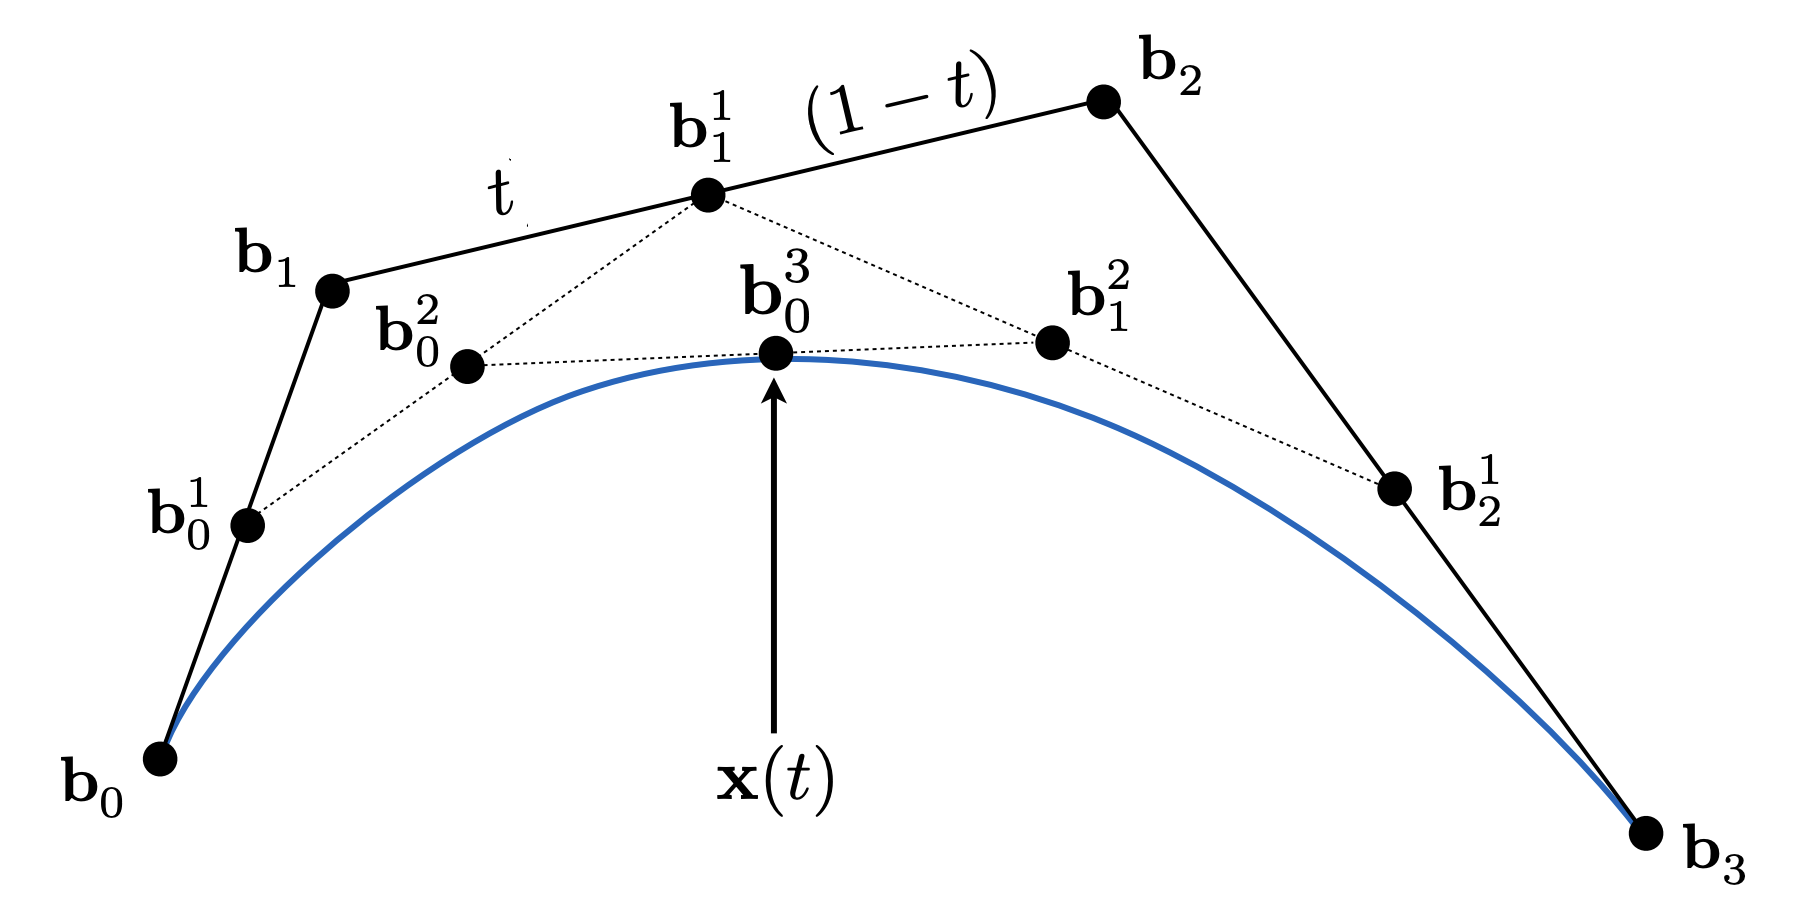
\includegraphics[scale=.15]{beisaier4.png}
\caption{四个控制点确定贝塞尔曲线的画法}
\label{fig:beisaier4}
\end{figure}

\subsection{贝塞尔曲线的数学表示}

通过上一节我们可以看出贝塞尔曲线的画法是类似于递归的方式画出的. 我们也知道贝塞尔曲线上的点只和参数$t$有关. 因此我们可以得到曲线的数学表示. 
\begin{equation}
	b^n=b_0^n=\sum_{j=0}^nb_jB_j^n(t)
\end{equation}
其中$B_j^n(t)$是Bernstein多项式, 它是$(t+(1-t))^n$二项分布的第$n$项展开: 
\begin{equation}
	B_j^n(t)=\binom{n}{i}t^i(1-t)^{n-i}
\end{equation}

在三维情况下, 公式不变. 所有的点变成三维空间上的点进行计算即可. 

\subsection{贝塞尔曲线的性质}
贝塞尔曲线满足以下性质: 
\begin{enumerate}
	\item 贝塞尔曲线必须过起点和终点; 
	\item 在四个控制点的情况下, 贝塞尔曲线在起点的切线是$b'(0)=3(b_1-b_0)$, 终点的切线是$b'(1)=3(b_3-b_2)$; 
	\item 对贝塞尔曲线做仿射变换生成的曲线等同于对贝塞尔曲线的控制点做仿射变换后再生成的贝塞尔曲线, 这个规律不适用于投影变换; 
	\item 凸包性质. 画出的贝塞尔曲线一定在控制点所形成的凸包内. 凸包是能够包围所有点的最小凸多边形. 
\end{enumerate}

\subsection{逐段定义贝塞尔曲线}
当我们使用过多的控制点定义一条曲线时, 曲线会变得比较平滑, 并且不便控制. 因此我们一般使用逐段的方式定义贝塞尔曲线. 我们每次使用4个控制点. 我们会把前两个点和后两个点各看作一个控制杆来控制整个曲线. 这和Photoshop中的钢笔工具是一致的. 

对于逐段的贝塞尔曲线, 我们需要保证其连续性, 我们对连续性有以下定义: 
\begin{itemize}
	\item 如果两条分段曲线的起点和终点重合, 那么称为C0连接; 
	\item 在上面的情况下, 如果第一条曲线终点的切线和第二条曲线起点的切线一样, 那么称为C1连接; 
	\item 在上面的情况下, 如果这两个点的n阶导数相同, 那么称为Cn连接. 
\end{itemize}
一边情况下C1连接就显得足够光滑. 在某些特殊情况下我们需要更高阶的连续. 

\subsection{样条曲线}
\textbf{样条曲线 (Split Curve) }可以形象地理解为在定义了多个控制点后, 在这些控制点上固定一个有弹性的木条形成的曲线. 在任何一点上不论几阶导数都是连续的. 最常见的样条曲线称为B-样条 (Basis) . 

\section{曲面}
我们可以通过曲线的定义扩展出\textbf{曲面 (Surface) }的定义. 

\subsection{贝塞尔曲面}
贝塞尔曲面的计算类似于双线性插值的过程. 我们使用$4\times 4$个点形成贝塞尔曲面. 首先, 我们在每一行生成4条贝塞尔曲线, 接下来在4条贝塞尔曲线上找到相同时刻对应的4个点生成一条新的贝塞尔曲线. 这些贝塞尔曲线的集合形成了贝塞尔曲面. 对于贝塞尔曲面, 我们需要两个变量$u,v$对其进行数学表示. 

\chapter{网格操作}
我们会对模型的网格进行一些操作来达到我们使用的目的. 基本的操作包括网格细分 (Mesh Subdivision) , 网格简化 (Mesh Simplify) 以及网格正则化 (Mesh Regularization) . 本章将会对前两个操作进行讲解. 网格正则化指的是将三角形的平面变成接近于正三角形的一种操作. 

\section{网格细分}
\textbf{网格细分 (Mesh Subdivision) }会增加更多的三角形面数量, 可以看到更多的细节. 细分分为两步, 第一步是增加三角形的数量, 第二步是计算三角形的位置. 

\subsection{Loop细分}
Loop细分适用于只有三角形面的模型. 首先, 每一个三角形面上我们依次连接三条边中点划分为四个新的三角形面. 每条边上的中点称为\textbf{新顶点 (New Vertex) }, 原来三角形面上的三个顶点称为\textbf{旧顶点 (Old Vertex) }. 

对于新顶点和旧顶点, 我们采用不同的位置计算方法: 

对于非边界上的新顶点, 一定被两个三角形面共享. 我们假设共享边的顶点是$A,B$, 非共享边的两个顶点是$C,D$, 那么新顶点的位置是: 
\begin{equation}
	\frac{3}{8}(A+B)+\frac{1}{8}(C+D)
\end{equation}

对于旧顶点, 假设顶点的度为$n$, 原顶点为$O$, 周围顶点位置之和为$S$, 那么新的顶点位置是: 
\begin{equation}
	(1-n\cdot u)\ O+u\ S
\end{equation}
这里, $u=\frac{3}{8n}$. 

顶点的计算是一个加权平均的过程, 会使整个模型更加的平滑. 

\subsection{Catmull-Clerk细分}
Catmull-Clerk细分适用于某些面是非三角形的时候进行细分. 我们做出以下定义, 如果一个面是四边形, 那么称为四边形面, 反之为非四边形面. 任何一个度不是$4$的点都称为奇异点, 反之为非奇异点. 

每一次细分我们都在每一条边的中点产生新的顶点, 并在每一个面上引入一个中点, 将面的中点和边上的中点相连, 这就是一次细分操作. 这样的细分操作满足一下规律: 
\begin{enumerate}
	\item 在第一次细分后, 所有原本是非四边形内部都会引入奇异点, 并且所有的面都变成了四边形面; 
	\item 之后的细分, 不会再引入新的奇异点, 所有的面都是四边形面. 
\end{enumerate}

\begin{figure}[H]
	\centering
	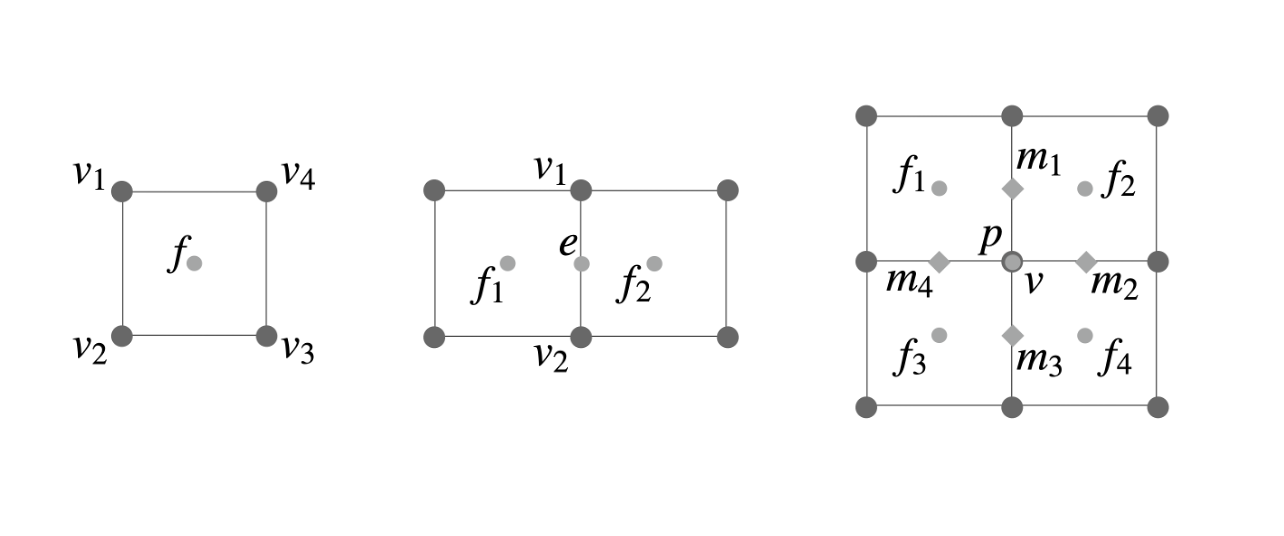
\includegraphics[scale=.4]{xifen.png}
	\caption{Catmull-Clerk细分中, 面心, 边上的中心以及旧顶点位置的计算}
	\label{fig:xifen}
\end{figure}
这样, 对于出现各种形状的面, 我们都可以进行细分. 这些点新的位置的计算方式如下: 
对于面心的点$f$, 计算方式为: 
\begin{equation}
	f=\frac{v_1+v_2+v_3+v_4}{4}
\end{equation}

对于边上新生成的中点$e$, 计算公式为:
\begin{equation}
	e=\frac{v_1+v_2+f_1+f_2}{4}
\end{equation}

对于旧顶点$v$, 新的位置的计算公式为: 
\begin{equation}
	v=\frac{f_1+f_2+f_3+f_4+2(m_1+m_2+m_3+m_4)+4p}{16}
\end{equation}

\section{网格简化}
\textbf{网格简化 (Mesh Simplify) }通过减少模型的面数简化模型. 对于一个模型, 我们可以通过构造不同的层级, 在不同的情况下选择不同的模型. 

我们使用\textbf{坍缩 (Collapsing) }的方式进行网格简化. 我们将边坍缩变成一个点. 我们希望这个点和旧顶点连接后与之前的形状差不多, 因此我们引入二次误差度量 (Quadric Error Metrics) 来度量任意一点与旧顶点连接后与原来的相似程度, 并选择最小值作为结果. 

在模型中, 当我们进行坍缩的时候, 我们会对所有可以坍缩的点进行排序, 每一次探索误差最小的点后, 更新这个点周围的点新的误差值. 这里采用堆或者优先队列的方式进行实现. 

网格简化是一种贪心算法, 我们使用局部的最优解并认为是全局最优的结果. 
